\documentclass[a4paper]{article}
\usepackage[pdftex]{graphicx}
\usepackage[utf8]{inputenc}
\usepackage{enumerate}
\usepackage{siunitx}
\sisetup{locale=DE}
\usepackage{icomma}
\usepackage{amssymb}
\usepackage{tikz}
\usepackage{href-ul}
\hypersetup{
	colorlinks=true,
	linkcolor=blue,
	urlcolor=blue}
\usepackage{geometry}
\geometry{a4paper, top=15mm, left=15mm, right=15mm, bottom=15mm,
	headsep=10mm, footskip=12mm}

\begin{document}
	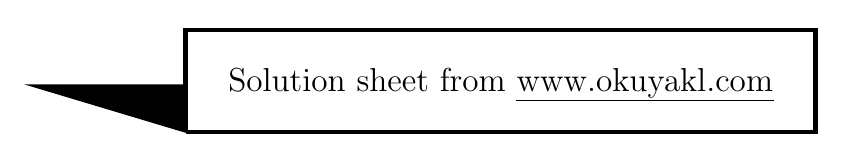
\begin{tikzpicture}(10,3)
		\draw[ultra thick](2,0) --(10,0) -- (10,1.3) --(2,1.3) -- (2,0);
		\draw[fill=black](2,0)-- (0,.6) -- (2,.6) -- (2,0);
		\node at (6,.6) {\large Solution sheet from \href{http://www.okuyakl.com}{www.okuyakl.com}};
	\end{tikzpicture}
	\vspace{0.5 cm}
	
	\noindent{\bf Task 1. a)}\\
	The centripetal force must be equal to or greater than the weight. Then the angular velocity follows:
	$$
	\renewcommand{\arraystretch}{2}
	\begin{array}{rcll}
		m \omega^2 r &\ge& m g \\
		\omega &\ge& \sqrt{g \over r} & \stackrel{r=\SI{6,0}{\meter}}{\Longrightarrow} \quad \omega = \SI{1,27}{1 \ over s}
	\end{array}
	$$
	\vspace{0.5 cm}
	
	\noindent{\bf Task 1. b)}\\
	$$f = {\omega \over 2 \pi } = {1 \over 2 \pi } \cdot \sqrt{g \over r} \quad \stackrel{r=\SI{6,0}{\meter} }{\Longrightarrow} \quad f = \SI{0.20}{\hertz}$$
	\vspace{0.5 cm}
	
	\noindent{\bf Task 1. c)}\\
	$$ T = {1\over f} = 2\pi \cdot \sqrt{r \over g} \quad \stackrel{r=\SI{6,0}{\meter}}{\Longrightarrow} \quad T = \SI{4,9}{\second}$$
	\vspace{0.5 cm}
	
	\noindent{\bf Task 1. d)}\\
	$$ v = \omega r = \sqrt{gr} \quad \stackrel{r=\SI{6,0}{\meter}}{\Longrightarrow} \quad v = \SI{7,7}{\meter \over\second}$$
	\vspace{0.5 cm}
	
	\noindent{\bf Task 2.}\\
	At point A the centripetal force must be greater than or equal to the weight, so the path speed at this point is:
	$$v_A = \sqrt{gr}$$
	And so for the kinetic energy here:
	$$E_{kinA}={1 \over 2 } m\cdot g \cdot r$$
	At the lower starting point the kinetic energy is higher, namely by the amount of the potential energy:
	$$E_{kinS}=E_{kinA}+E_{pot}={1 \over 2 } m g \cdot r + m g\cdot 2r= 2.5 ~m g r $$
	We equate this with the tension energy of the spring:
	$$
	\renewcommand{\arraystretch}{2}
	\begin{array}{rcll}
		E_{Sp}&=&{1\over 2} D s^2 = 2.5 ~mgr\\
		s^2 &=& 5.0 {mgr \over D} \\
		s &=& \sqrt{5.0 {mgr \over D}} &= \SI{0.30}{\meter}
	\end{array}
	$$
	\vspace{0.5 cm}
	
	\newpage
	\noindent{\bf Task 3. a)}\\
	\noindent
	\begin{minipage}{0.5\textwidth}
		The force rectangle that is created by the centrifugal force and the weight applies to the cyclist. For the angle $\alpha$ the following applies:
		$$
		\renewcommand{\arraystretch}{2}
		\begin{array}{rcll}
			\tan \alpha &=& { F_Z \over F_G}\\
			\tan \alpha &=& {m v^2 \over m g r} \\
			\tan \alpha &=& { v^2 \over g r} \\
			\tan \alpha &=& { ( \SI{6,0}{\meter\over \second})^2 \over \SI{9,81}{\meter\over {\second^2}} \cdot \SI{30}{\meter}}\\
			\tan \alpha &=& 0.122 \\
			\alpha &=& \SI{7,0}{\degree}
		\end{array}
		$$
	\end{minipage}
	\hfill
	\begin{minipage}{0.5\textwidth}
		\includegraphics[width=7 cm]{fara415}
	\end{minipage}
	\vspace{0.5 cm}
	
	\noindent{\bf Task 3. b)}\\
	The coefficient of static friction $\mu$ corresponds to the maximum ratio of horizontal to vertical force, which here is exactly $\tan \alpha $:
	$$ \tan \alpha_{max} = 0.7 \quad \Rightarrow \quad \alpha_{max}= \SI{35}{\degree}$$
	\vspace{0.5 cm}
	
	\noindent{\bf Task 4.}\\
	We set the static friction force equal to the centripetal force:
	$$
	\renewcommand{\arraystretch}{2}
	\begin{array}{rclll}
		F_R &=& F_Z \\
		m \cdot {v^2 \over r} &=& \mu \cdot m g \\
		v &=& \sqrt{\mu \cdot g r} &= \sqrt{0.80 \cdot \SI{9.81}{\meter\over {\second^2}} \cdot \SI{50}{ \meter}} &=\SI{20}{\meter\over\second}
	\end{array}
	$$
	\vspace{0.5 cm}
	
	\noindent{\bf Task 5.}\\
	For the calculation we choose the approach as in task 3:
	$$
	\renewcommand{\arraystretch}{2}
	\begin{array}{rcll}
		\tan \alpha &=& { F_Z \over F_G}\\
		\tan \alpha &=& { v^2 \over g R} \\
		v &=& \sqrt{\tan\alpha \cdot g R}
	\end{array}
	$$
	Here R is the entire radius:
	$$R=r+l\cdot \sin\alpha = 3.0 + 3.5 \cdot \sin \SI{20}{\degree} = \SI{4.2}{\meter}$$
	We substitute and get for $v$:
	$$\Rightarrow \quad v = \sqrt{\tan \SI{20}{\degree}\cdot \SI{9,81}{\meter \over {\second^2}} \cdot \SI{4, 2}{\meter}}=\SI{3,9}{\meter\over\second}$$
	The orbital period T is:
	$$T ={2 \pi R \over v} = \SI{6,8}{\second}$$
	
	\begin{center}
		\includegraphics[width=7 cm]{../../viecher/eendcomic.pdf}
		
		Here you can go back to the \href{https://www.okuyakl.de/phys/p10krbL415/ae415.pdf}{task sheet}
	\end{center}
	
\end{document}